\subsubsection{\stid{6.02} LLNL ATDM: RAJA, UMPIRE, and CHAI}


\paragraph{Overview}

RAJA, CHAI, and Umpire are providing software libraries that enable
application and library developers to meet advanced architecture
portability challenges. The project goals are to enable writing
performance portable computational kernels and coordinate complex
heterogeneous memory resources among components in a large integrated
application. These libraries enhance developer productivity by insulating
them from much of the complexity associated with parallel programming
model usage and system-specific memory concerns.

The software products provided by this project are three complementary
and interoperable libraries:

\begin{enumerate}

\item {\bf RAJA}: Software abstractions that enable C++ developers to write
    performance portable (i.e., single-source) numerical kernels (loops).

\item {\bf CHAI}: C++ ``managed array'' abstractions that enable transparent
    and automatic copying of application data to memory spaces at run
    time as needed based on RAJA execution contexts.

\item {\bf Umpire}: A portable memory resource management library that provides
    a unified high-level API in C++, C and FORTRAN for resource
    discovery, memory provisioning, allocation, transformation, and
    introspection.

\end{enumerate}

Capabilities delivered by these software efforts are needed to manage the
diversity and uncertainty associated with current and future HPC
architecture design and software support. Moving forward, ECP
applications and libraries need to achieve performance portability:
without becoming bound to particular (potentially limiting) hardware or
software technologies, by insulating numerical algorithms from
platform-specific data and execution concerns, and without major
disruption as new machine, programming models, and vendor software become
available.

These libraries in development in this project are currently used in
production ASC applications at Lawrence Livermore National Laboratory
(LLNL) and receive most of their support from the LLNL national security
application project. They are also being used or being explored/adopted
by several ECP application and library projects, including: LLNL ATDM
application, GEOS (Subsurface), SW4 (EQSIM), MFEM (CEED co-design),
DevilRay (Alpine), and SUNDIALS.


\paragraph{Key Challenges} \leavevmode \\

Exascale machines are expected to be very diverse, with different GPU,
threading, memory models, and node architectures.  A parallelization
strategy that works well for one machine may not work well for another,
but application developers cannot afford to develop multiple versions of
their code for each machine they support.  Rather, the application must
be written using higher-level abstractions, and adapted at a lower level,
with minimal programmer effort, to specific machines.  RAJA, Umpire, and
CHAI addres this by giving applicationst the flexibility to adapt and
tune for many target machines, using the same high level kernel
formulations.  In other words they separate the concerns of performance
and correctness and avoid a combinatorial explosion of code versions for
the exascale ecosystem.

In addition to performance portability, RAJA, Umpire, and CHAI
specifically target the porting issues faced by legacy codes.  Where
other performnance portability frameworks may require a larger up-front
investment in data structures and code restructuring, RAJA, Umpire, and
CHAI are non-invasive and allow codes to adopt strategies for loop
parallelism, data layout tuning, and memory management separately.
Legacy applicaitons need not adopt all three at once; they can gradually
integrate each framework, at their own pace, with a minimal set of code
modifications.

\paragraph{Solution Strategy} \leavevmode \\

RAJA, Umpire, and CHAI leverage the abstraction mechanisms available in
modern C++ (C++11 and higher) compilers, such as Lambdas, policy
templates, and constructor/destructor (RAII) patterns for resource
management.  They aim to provide performance portability at the {\it
library} level, and they do not require special support from compilers.
Targeting this level of the software stack gives DOE developers the
flexibility to leverage standard parallel programming models like CUDA
and OpenMP, without strictly {\it depending} on robust compiler support
for these APIs.  If necessary features are unavailable in compilers,
library authors are not dependent on vendors for support, and they do not
need to wait for these programming models to be fully implemented.  These
libraries allow applications to work correctly and performantly even if
some functionality from OpenMP, CUDA, threading, etc. is missing.


\paragraph{Recent Progress} \leavevmode \\

\begin{figure}[htb]
\centering
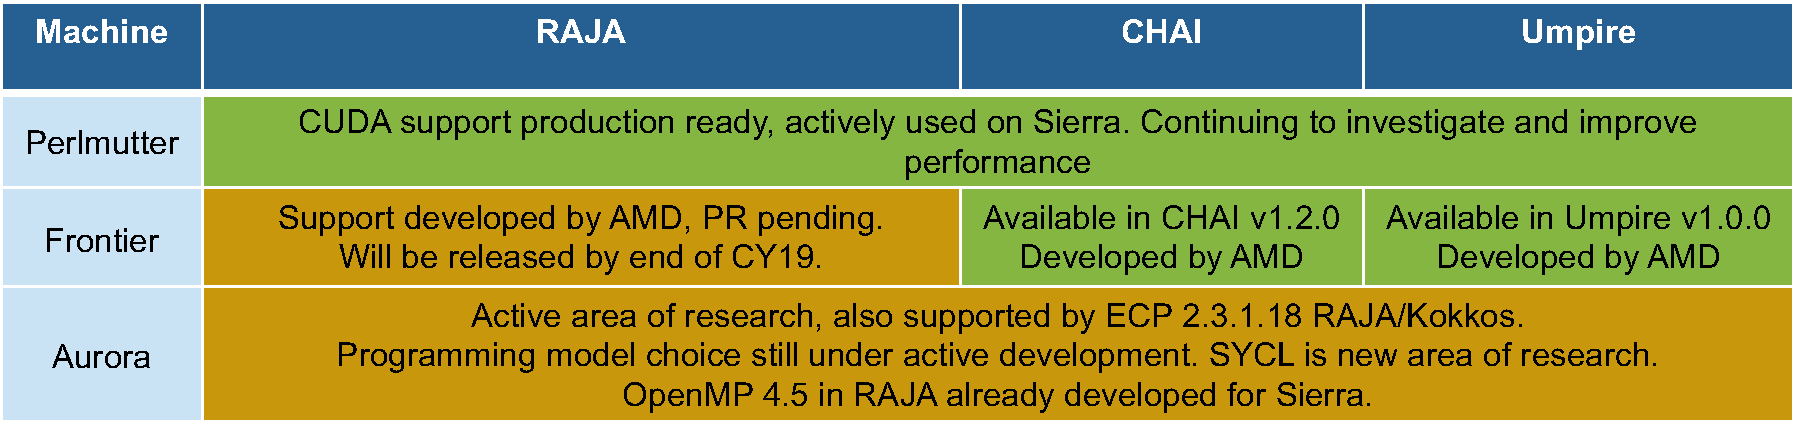
\includegraphics[width=\textwidth]{projects/2.3.6-NNSA/2.3.6.02-LLNL-ATDM/raja-umpire-chai-support}
\caption{
Status of RAJA, Umpire, and CHAI support for exascale platforms.
}
\end{figure}

{\bf RAJA}
\begin{itemize}
\item Comprehensive support for Sierra (Power9/Volta),
      including multi-dimensional kernel dispatch.
\item enabled first full-system run on Sierra (16k GPUs, 97B elements)
\item Added support for atomic operations on GPU devices.
\item Integrated with GEOS, SW4, SUNDIALS, DevilRay, and LLNL ATDM.
\end{itemize}

{\bf Umpire}
\begin{itemize}
\item Developed support for Sierra (Power9 + Volta) systems, incl. allocation
      on CPU, GPU, unified, and “pinned” memory resources; copying bt/w any
      resources; fast memory pools; CUDA ``memory advice''.
\item Completed integration with multiple LLNL ASC applications and libraries,
      SW4, GEOS, and DevilRay. Began integration with LLNL ATDM application.
\end{itemize}

{\bf CHAI}
\begin{itemize}
\item Developed Umpire-based backend for CHAI which adds additional flexibility
      and capability.
\item Add option to pass specific Umpire objects (like pooled allocators) to
      CHAI arrays to improve application performance.
\item Integrated with GEOS (ECP App Subsurface) application.
\end{itemize}

\paragraph{Next Steps}  \leavevmode \\

Work in FY20–FY23 will focus on supporting El Capitan and other
exascale-class systems available during this time frame. Additional work
will support ASC and ATDM applications performance production runs on
Sierra and integrating Umpire into additional LLNL WSC software
components like Sidre, a simulation data store supported under the Axom
project in the LLNL national security application project.

\begin{itemize}
\item Support LLNL ASC and ATDM applications with Sierra production runs
\item Add El Capitan support to RAJA, CHAI, and Umpire
\item Integrate Umpire with Sidre
\item Support LLNL ASC and ATDM applications with transition to exascale
      systems
\end{itemize}
